%!TeX spellcheck = en_GB
% Die erste (unkommentierte) Zeile im Dokument legt immer die
% Dokumentklasse fest
\documentclass{scrartcl} 

% Präambel:
% Einbinen von zusätzlichen Paketen. Falls für eine Datei keine Endung
% explizit angegeben wird, benutzt LaTeX '.tex'. Im Folgenden wird
% also die Datei 'edv_pakete.tex' eingebunden.
\input{edv_pakete}


% Verzeichnisse mit Abbildungen; kann gestrichen werden,
% falls Sie dies schon in edv_pakete.tex definiert haben:
%\graphicspath{{../report}}

\addbibresource{refs.bib} %Hinzufügen einer Literaturdatenbank aus dem angegebenen Verzeichnis

% Titel, Autor und Datum
\title{Computational Physics}
\subtitle{Exercise 6}
\date{\today}
\author{Christiane Groß, Nico Dichter}

% Jetzt startet das eigentliche Dokument
\begin{document}
	\maketitle
	
\section{Theory}

\section{Results}
\subsection{Accuracy}

We check the numerical accuracy of our results by plotting $F(\vec{q}^2)$ for several $\vec{q}^2$ for different nx, see fig.~\ref{fig:accuracy}. We see that for very small nx the results change rapidly and grow bigger for bigger nx, but a plateau is reached very soon, at nx=5. For bigger nx we cannot see a change at the plotted resolution. 

\begin{figure}[htbp]
	\input{stability.tex}
	\caption{Results for $\Lambda=1200\si{\mega\electronvolt}$, different $\vec{q}$ and different nx}
	\label{fig:accuracy}
\end{figure}

further comparison: table nx, F(1)

\subsection{Normalization and Radius}
The deviation $F(0)-1$ is plotted for the different values of the cut-off-energy in fig.~\ref{fig:fofzero}. We see that for all chosen $\lambda$ the deviation is less than one part per million and we do not see any trend in the data to either rise or fall for changing $\Lambda$.
  
  
\begin{figure}[htbp]
	% GNUPLOT: LaTeX picture with Postscript
\begingroup
  \makeatletter
  \providecommand\color[2][]{%
    \GenericError{(gnuplot) \space\space\space\@spaces}{%
      Package color not loaded in conjunction with
      terminal option `colourtext'%
    }{See the gnuplot documentation for explanation.%
    }{Either use 'blacktext' in gnuplot or load the package
      color.sty in LaTeX.}%
    \renewcommand\color[2][]{}%
  }%
  \providecommand\includegraphics[2][]{%
    \GenericError{(gnuplot) \space\space\space\@spaces}{%
      Package graphicx or graphics not loaded%
    }{See the gnuplot documentation for explanation.%
    }{The gnuplot epslatex terminal needs graphicx.sty or graphics.sty.}%
    \renewcommand\includegraphics[2][]{}%
  }%
  \providecommand\rotatebox[2]{#2}%
  \@ifundefined{ifGPcolor}{%
    \newif\ifGPcolor
    \GPcolortrue
  }{}%
  \@ifundefined{ifGPblacktext}{%
    \newif\ifGPblacktext
    \GPblacktextfalse
  }{}%
  % define a \g@addto@macro without @ in the name:
  \let\gplgaddtomacro\g@addto@macro
  % define empty templates for all commands taking text:
  \gdef\gplbacktext{}%
  \gdef\gplfronttext{}%
  \makeatother
  \ifGPblacktext
    % no textcolor at all
    \def\colorrgb#1{}%
    \def\colorgray#1{}%
  \else
    % gray or color?
    \ifGPcolor
      \def\colorrgb#1{\color[rgb]{#1}}%
      \def\colorgray#1{\color[gray]{#1}}%
      \expandafter\def\csname LTw\endcsname{\color{white}}%
      \expandafter\def\csname LTb\endcsname{\color{black}}%
      \expandafter\def\csname LTa\endcsname{\color{black}}%
      \expandafter\def\csname LT0\endcsname{\color[rgb]{1,0,0}}%
      \expandafter\def\csname LT1\endcsname{\color[rgb]{0,1,0}}%
      \expandafter\def\csname LT2\endcsname{\color[rgb]{0,0,1}}%
      \expandafter\def\csname LT3\endcsname{\color[rgb]{1,0,1}}%
      \expandafter\def\csname LT4\endcsname{\color[rgb]{0,1,1}}%
      \expandafter\def\csname LT5\endcsname{\color[rgb]{1,1,0}}%
      \expandafter\def\csname LT6\endcsname{\color[rgb]{0,0,0}}%
      \expandafter\def\csname LT7\endcsname{\color[rgb]{1,0.3,0}}%
      \expandafter\def\csname LT8\endcsname{\color[rgb]{0.5,0.5,0.5}}%
    \else
      % gray
      \def\colorrgb#1{\color{black}}%
      \def\colorgray#1{\color[gray]{#1}}%
      \expandafter\def\csname LTw\endcsname{\color{white}}%
      \expandafter\def\csname LTb\endcsname{\color{black}}%
      \expandafter\def\csname LTa\endcsname{\color{black}}%
      \expandafter\def\csname LT0\endcsname{\color{black}}%
      \expandafter\def\csname LT1\endcsname{\color{black}}%
      \expandafter\def\csname LT2\endcsname{\color{black}}%
      \expandafter\def\csname LT3\endcsname{\color{black}}%
      \expandafter\def\csname LT4\endcsname{\color{black}}%
      \expandafter\def\csname LT5\endcsname{\color{black}}%
      \expandafter\def\csname LT6\endcsname{\color{black}}%
      \expandafter\def\csname LT7\endcsname{\color{black}}%
      \expandafter\def\csname LT8\endcsname{\color{black}}%
    \fi
  \fi
    \setlength{\unitlength}{0.0500bp}%
    \ifx\gptboxheight\undefined%
      \newlength{\gptboxheight}%
      \newlength{\gptboxwidth}%
      \newsavebox{\gptboxtext}%
    \fi%
    \setlength{\fboxrule}{0.5pt}%
    \setlength{\fboxsep}{1pt}%
\begin{picture}(8502.00,5668.00)%
    \gplgaddtomacro\gplbacktext{%
      \csname LTb\endcsname%
      \put(1342,704){\makebox(0,0)[r]{\strut{}$-1\times10^{-6}$}}%
      \put(1342,1879){\makebox(0,0)[r]{\strut{}$-5\times10^{-7}$}}%
      \put(1342,3054){\makebox(0,0)[r]{\strut{}$0$}}%
      \put(1342,4228){\makebox(0,0)[r]{\strut{}$5\times10^{-7}$}}%
      \put(1342,5403){\makebox(0,0)[r]{\strut{}$1\times10^{-6}$}}%
      \put(1474,484){\makebox(0,0){\strut{}$300$}}%
      \put(2211,484){\makebox(0,0){\strut{}$400$}}%
      \put(2948,484){\makebox(0,0){\strut{}$500$}}%
      \put(3684,484){\makebox(0,0){\strut{}$600$}}%
      \put(4421,484){\makebox(0,0){\strut{}$700$}}%
      \put(5158,484){\makebox(0,0){\strut{}$800$}}%
      \put(5895,484){\makebox(0,0){\strut{}$900$}}%
      \put(6631,484){\makebox(0,0){\strut{}$1000$}}%
      \put(7368,484){\makebox(0,0){\strut{}$1100$}}%
      \put(8105,484){\makebox(0,0){\strut{}$1200$}}%
    }%
    \gplgaddtomacro\gplfronttext{%
      \csname LTb\endcsname%
      \put(176,3053){\rotatebox{-270}{\makebox(0,0){\strut{}$F(\vec{q}^2)/\si{\femto\meter^2}-1$}}}%
      \put(4789,154){\makebox(0,0){\strut{}$\Lambda/\si{\mega\electronvolt}$}}%
    }%
    \gplbacktext
    \put(0,0){\includegraphics{fofzero}}%
    \gplfronttext
  \end{picture}%
\endgroup

	\caption{$F(0)$ for different $\Lambda$, nx=20}
	\label{fig:fofzero}
\end{figure}

We calculated the radius by fitting a polynomial of third order to the calculated data: $F(\vec{q}^2)=a+b\cdot \vec{q}^2+c\cdot\vec{q}^4+d\cdot\vec{q}^6$. We did the fit with the gnuplot fit-routine, which internally uses the nonlinear least-squares Marquardt-Levenberg algorithm~\cite[p. 74]{gnuplotdoc}. From this we calculated $\sqrt{\langle r^2\rangle}=\sqrt{-6b}$ and determined the error using Gaussian error propagation. The results for $\sqrt{\langle r^2\rangle}$ are plotted in fig.~\ref{fig:radius}, together with the results given in the lecture.

\begin{figure}[htbp]
	\input{radius.tex}
	\caption{$\sqrt{\langle r^2\rangle}$ for different $\Lambda$, nx=20}
	\label{fig:radius}
\end{figure}

Qualitatively, both show the same behaviour of having the largest value at $\Lambda=300\si{\mega\electronvolt}$, the dipping to a minimum at $\Lambda=500\si{\mega\electronvolt}$, and then rising slowly. However, all of our measurements are about $.02\si{\femto\meter}$, or 1\%, below the data points from the lecture.

\subsection{Form Factor at different Cut-off-energies}

\begin{figure}[htbp]
	% GNUPLOT: LaTeX picture with Postscript
\begingroup
  \makeatletter
  \providecommand\color[2][]{%
    \GenericError{(gnuplot) \space\space\space\@spaces}{%
      Package color not loaded in conjunction with
      terminal option `colourtext'%
    }{See the gnuplot documentation for explanation.%
    }{Either use 'blacktext' in gnuplot or load the package
      color.sty in LaTeX.}%
    \renewcommand\color[2][]{}%
  }%
  \providecommand\includegraphics[2][]{%
    \GenericError{(gnuplot) \space\space\space\@spaces}{%
      Package graphicx or graphics not loaded%
    }{See the gnuplot documentation for explanation.%
    }{The gnuplot epslatex terminal needs graphicx.sty or graphics.sty.}%
    \renewcommand\includegraphics[2][]{}%
  }%
  \providecommand\rotatebox[2]{#2}%
  \@ifundefined{ifGPcolor}{%
    \newif\ifGPcolor
    \GPcolortrue
  }{}%
  \@ifundefined{ifGPblacktext}{%
    \newif\ifGPblacktext
    \GPblacktextfalse
  }{}%
  % define a \g@addto@macro without @ in the name:
  \let\gplgaddtomacro\g@addto@macro
  % define empty templates for all commands taking text:
  \gdef\gplbacktext{}%
  \gdef\gplfronttext{}%
  \makeatother
  \ifGPblacktext
    % no textcolor at all
    \def\colorrgb#1{}%
    \def\colorgray#1{}%
  \else
    % gray or color?
    \ifGPcolor
      \def\colorrgb#1{\color[rgb]{#1}}%
      \def\colorgray#1{\color[gray]{#1}}%
      \expandafter\def\csname LTw\endcsname{\color{white}}%
      \expandafter\def\csname LTb\endcsname{\color{black}}%
      \expandafter\def\csname LTa\endcsname{\color{black}}%
      \expandafter\def\csname LT0\endcsname{\color[rgb]{1,0,0}}%
      \expandafter\def\csname LT1\endcsname{\color[rgb]{0,1,0}}%
      \expandafter\def\csname LT2\endcsname{\color[rgb]{0,0,1}}%
      \expandafter\def\csname LT3\endcsname{\color[rgb]{1,0,1}}%
      \expandafter\def\csname LT4\endcsname{\color[rgb]{0,1,1}}%
      \expandafter\def\csname LT5\endcsname{\color[rgb]{1,1,0}}%
      \expandafter\def\csname LT6\endcsname{\color[rgb]{0,0,0}}%
      \expandafter\def\csname LT7\endcsname{\color[rgb]{1,0.3,0}}%
      \expandafter\def\csname LT8\endcsname{\color[rgb]{0.5,0.5,0.5}}%
    \else
      % gray
      \def\colorrgb#1{\color{black}}%
      \def\colorgray#1{\color[gray]{#1}}%
      \expandafter\def\csname LTw\endcsname{\color{white}}%
      \expandafter\def\csname LTb\endcsname{\color{black}}%
      \expandafter\def\csname LTa\endcsname{\color{black}}%
      \expandafter\def\csname LT0\endcsname{\color{black}}%
      \expandafter\def\csname LT1\endcsname{\color{black}}%
      \expandafter\def\csname LT2\endcsname{\color{black}}%
      \expandafter\def\csname LT3\endcsname{\color{black}}%
      \expandafter\def\csname LT4\endcsname{\color{black}}%
      \expandafter\def\csname LT5\endcsname{\color{black}}%
      \expandafter\def\csname LT6\endcsname{\color{black}}%
      \expandafter\def\csname LT7\endcsname{\color{black}}%
      \expandafter\def\csname LT8\endcsname{\color{black}}%
    \fi
  \fi
    \setlength{\unitlength}{0.0500bp}%
    \ifx\gptboxheight\undefined%
      \newlength{\gptboxheight}%
      \newlength{\gptboxwidth}%
      \newsavebox{\gptboxtext}%
    \fi%
    \setlength{\fboxrule}{0.5pt}%
    \setlength{\fboxsep}{1pt}%
\begin{picture}(8502.00,5668.00)%
    \gplgaddtomacro\gplbacktext{%
      \csname LTb\endcsname%
      \put(946,704){\makebox(0,0)[r]{\strut{}$-0.2$}}%
      \put(946,1487){\makebox(0,0)[r]{\strut{}$0$}}%
      \put(946,2270){\makebox(0,0)[r]{\strut{}$0.2$}}%
      \put(946,3054){\makebox(0,0)[r]{\strut{}$0.4$}}%
      \put(946,3837){\makebox(0,0)[r]{\strut{}$0.6$}}%
      \put(946,4620){\makebox(0,0)[r]{\strut{}$0.8$}}%
      \put(946,5403){\makebox(0,0)[r]{\strut{}$1$}}%
      \put(1078,484){\makebox(0,0){\strut{}$0$}}%
      \put(2207,484){\makebox(0,0){\strut{}$20$}}%
      \put(3336,484){\makebox(0,0){\strut{}$40$}}%
      \put(4464,484){\makebox(0,0){\strut{}$60$}}%
      \put(5593,484){\makebox(0,0){\strut{}$80$}}%
      \put(6722,484){\makebox(0,0){\strut{}$100$}}%
    }%
    \gplgaddtomacro\gplfronttext{%
      \csname LTb\endcsname%
      \put(176,3053){\rotatebox{-270}{\makebox(0,0){\strut{}$F(\vec{q}^2)/\si{\femto\meter^2}$}}}%
      \put(3900,154){\makebox(0,0){\strut{}$q^2/\si{\femto\meter^{-2}}$}}%
      \put(7677,5293){\makebox(0,0){\strut{}$\Lambda/\si{\mega\electronvolt}$}}%
      \csname LTb\endcsname%
      \put(7514,5073){\makebox(0,0)[r]{\strut{}300}}%
      \csname LTb\endcsname%
      \put(7514,4853){\makebox(0,0)[r]{\strut{}400}}%
      \csname LTb\endcsname%
      \put(7514,4633){\makebox(0,0)[r]{\strut{}500}}%
      \csname LTb\endcsname%
      \put(7514,4413){\makebox(0,0)[r]{\strut{}600}}%
      \csname LTb\endcsname%
      \put(7514,4193){\makebox(0,0)[r]{\strut{}700}}%
      \csname LTb\endcsname%
      \put(7514,3973){\makebox(0,0)[r]{\strut{}800}}%
      \csname LTb\endcsname%
      \put(7514,3753){\makebox(0,0)[r]{\strut{}900}}%
      \csname LTb\endcsname%
      \put(7514,3533){\makebox(0,0)[r]{\strut{}1000}}%
      \csname LTb\endcsname%
      \put(7514,3313){\makebox(0,0)[r]{\strut{}1100}}%
      \csname LTb\endcsname%
      \put(7514,3093){\makebox(0,0)[r]{\strut{}1200}}%
    }%
    \gplbacktext
    \put(0,0){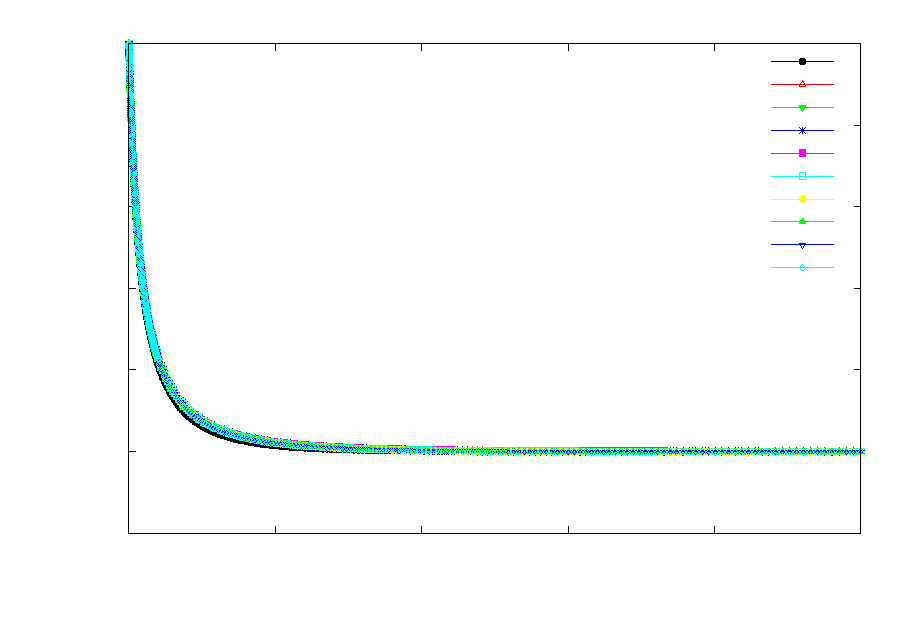
\includegraphics{formfactor}}%
    \gplfronttext
  \end{picture}%
\endgroup

	\caption{Form factor for different $\Lambda$}
	\label{fig:formfactor}
\end{figure}

\begin{figure}[htbp]
	\input{formfactorsmall.tex}
	\caption{Form factor for different $\Lambda$ and small momenta}
	\label{fig:formfactorsmall}
\end{figure}

\begin{figure}[htbp]
	\input{formfactorbig.tex}
	\caption{Form factor for different $\Lambda$ and big momenta}
	\label{fig:formfactorbig}
\end{figure}

\newpage
\listoffigures
\listoftables
\printbibliography
\end{document}
